%----------------------------------------------------------------------------------------
%	PACKAGES AND OTHER DOCUMENT CONFIGURATIONS
%----------------------------------------------------------------------------------------


\documentclass[12pt,openright,twoside,final]{report}
\usepackage{generators/imports}
\makeglossaries

\renewcommand*{\acronymname}{List of Acronyms and Abbreviations}
\renewcommand{\glsnamefont}[1]{\textbf{#1}}

%Create acronyms here.
\newacronym{saas}{SaaS}{Software as a Service}
\newacronym{kg}{KG}{Knowledge Graph}
\newacronym{kgc}{KGC}{Knowledge Graph Completion}
\newacronym{kge}{KGE}{Knowledge Graph Embedding}
\newacronym{vcs}{VCS}{Version Control System}
\newacronym{rdf}{RDF}{Resource Description Framework}
\newacronym{w3c}{W3C}{World Wide Web Consortium}
\newacronym{dls}{DLs}{Description logics}
\newacronym{dl}{DL}{Description Logic}
\newacronym{una}{UNA}{Unique Name Assumption}
\newacronym{owl}{OWL}{Web Ontology Language}
\newacronym{rnn}{RNN}{Recurrent neural network}
\newacronym{fol}{FOL}{First Order Logic}
\newacronym{pl}{PL}{Propositional Logic}
%You can also do explanations.
\newglossaryentry{git}{name={Git},
    description={Git is a \gls{vcs} for tracking changes in computer files and coordinating work on those files among multiple people}}

\begin{document}
\begin{titlepage}

\newcommand{\HRule}{\rule{\linewidth}{0.5mm}} % Defines a new command for the horizontal lines, change thickness here

\center % Center everything on the page
 
%----------------------------------------------------------------------------------------
%	HEADING SECTIONS
%----------------------------------------------------------------------------------------

\textsc{\LARGE University of Bergen \\ Department of informatics}\\[1.5cm] % Name of your university/college

%----------------------------------------------------------------------------------------
%	TITLE SECTION
%----------------------------------------------------------------------------------------

\HRule \\[0.5cm]
\begin{Huge}
	\bfseries{Rule mining on extended knowledge graphs}\\[0.7cm] % Title of your document
\end{Huge}
\HRule \\[0.5cm]

%----------------------------------------------------------------------------------------
%	AUTHOR SECTION
%----------------------------------------------------------------------------------------

\large \emph{Author:} Johanna Jøsang\\
\large \emph{Supervisors:} Ana Ozaki and Ricardo Guimarães\\[2cm]

%----------------------------------------------------------------------------------------
%   LOGO SECTION
% 	This will require the graphicx package
%	Change the line to comment if you only want the UiB Logo
%	Logo for other faculties here: http://kapd.h.uib.no/profilmanual/99LastNed/99a_lastned.html
%----------------------------------------------------------------------------------------

\centerline{\includegraphics[scale=1.9]{figures/canvasWithFaculty}}
%\centerline{
\includegraphics[scale=0.15]{figures/canvas}}  %change for your faculty

%----------------------------------------------------------------------------------------
%	DATE SECTION
%----------------------------------------------------------------------------------------

{\large \monthyeardate\today}\\[3cm] % Date, change the \today to a set date if you want to be precise

%----------------------------------------------------------------------------------------
%	LOGO SECTION
%----------------------------------------------------------------------------------------

\vfill % Fill the rest of the page with whitespace

\end{titlepage}
 % This is the titlepage
\pagenumbering{roman}
%\cite{schlichtkrull2018modeling, vashishth2019composition} (for neural networks citation)
\begin{abstract} 

\noindent Knowledge graphs (KGs) have risen in both size and use over the past few years, and there are a range of approaches for evaluating information in them. Symbolic approaches, such as rule-based machine learning, offer an explainable way to determine the appropriateness of a new fact based on rules mined from the KG in question. Some of the most successful approaches for fact prediction in KGs today are knowledge graph embeddings (KGEs) that use deep neural networks, however, these lack the explainability of symbolic approaches. We would like to see how the extension of a KG using KGEs affects the rules mined from the KG. A set of rules is mined from a KG and compared with another set mined from an \textit{extended} version of said KG. The experiments examine three classical KGEs: TransE, DistMult, and ComplEx, and use the rule mining algorithm AMIE3. AMIE3 is treated as a black box during the experiment, as the study only evaluates factors playing a role in the KG-extension process, one of which is the choice of KGE. The experiments show that there can be considerable discrepancies in the rules mined based on the choice of KGE and that TransE leads to a substantial amount of nonsensical rules being mined.

\end{abstract}

\renewcommand{\abstractname}{Acknowledgements}
\begin{abstract}
    First and foremost, I would like to thank my two supervisors, Ana and Ricardo. Ana was, from the start, a fantastic guide for me in the field of academic research and taught me a lot about writing and publishing work. Ricardo was always eager to answer and discuss questions, and his attention to detail taught me a lot. A great thank you to both of you. You have given me more support through this master's than I could have hoped for.
	
	I would like to thank my fellow master's students that battled with me over the two years. The workload is not so heavy when you are in it together. Thank you John Isak, Hans Martin, Knut, Halvor, Mathias, Magnus, Emir and Oda. You have been a fantastic group to work with, and I wish you all the best in your future work/studies.
	
	My final thanks goes out to family and friends, who have helped me by listening to my thoughts and reviewing the thesis. Complicated ideas become tangible and manageable when you put the correct words to them. Thank you for helping me find them.
	
	\vspace{1cm}
	\hspace*{\fill}Johanna Jøsang\\ 
	\hspace*{\fill} 01 June, 2022
\end{abstract}
\newpage
\include{generators/tableOfContentsAndListings}
\pagenumbering{arabic}
\setcounter{page}{1}
\setlength{\parskip}{0.5cm plus4mm minus3mm}  

\chapter{Introduction}

Knowledge bases that are large and interesting are generally not complete. They may for example be extracted from natural language resources and may contain facts that are wrong or exhibit gaps in their knowledge. Most of the data that is present, however, is correct and hence implicitly contain meaningful rules. For example the Wikidata dataset that contains information about many individuals will implicitly contain the fact that siblings tend to have the same mother:
\[siblingOf(a, b) \wedge motherOf(c, a) \Rightarrow motherOf(c, b)\]
There will of course be exceptions to this rule, but generally it will hold. The rules describe information about relational data, and hence will only use binary predicates. The rules will also be Horn, meaning that any number of predicates may be used in the body of the rule, but only one predicate is implied in the rule. This form has useful properties in knowledge representation and reasoning. When extracting rules from knowledge graphs they therefore tend to be Horn rules on binary predicates.

While many KG embedding techniques are both accurate and scalable, one of the main issues with this approach in that results usually are not explainable \cite{bonatti2019knowledge}. Rule-based machine learning approaches provide an explanation in the form of the rules used to make a prediction.  Meilicke et al. showed that a rule-bases mined with AMIE+ are good competitors and often outperform embedding models \cite{ensemble}. This was caused by the fact that the standard benchmark datasets, such as WN18 and FB15k,  have a great deal of relational regularities, such as symmetry and equivalence. Meilicke et al. also compared the two approaches for triple prediction and found that they compliment each other. An ensemble of the two families of approaches gave better results than either of the two alone.

This work inspired the idea of using KG embedding models to improve rule-bases, or vice versa. After applying one KG completion technique, the other can be modeled on the improved KG, resulting in a better model. This can be done both ways, as shown in figure \ref{rule_based_and_embedding}. A rule-base as end-result was chosen, ultimately because it results in an explainable model. 

\begin{figure}[htp]
    \centering
    \includesvg[inkscapelatex=false,width=1\textwidth,keepaspectratio]{figures/intro/custergraf-nesten.svg}
    \caption[Figure representing the process.]{The two versions of KG improvement for better model creation. In the top version an embedding of the original KG is used to improve the graph, from which a rule base is mined. Red edges represent new links made by the models, which originally weren't present in the KG. The second part of the figure represents the same process, but with the rule base used to improve the KG, resulting in an embedding of the improved KG. }
    \label{rule_based_and_embedding}
\end{figure}

This thesis assumes that the reader is familiar with basic machine learning concepts, such as training, testing and overfitting. For an introduction or refresher to machine learning basics, chapter 5 in the book \textit{Deep Learning}, by Goodfellow et al. \cite{goodfellow} covers the topic quite well. The entire book is publicly available at \href{https://www.deeplearningbook.org/}{https://www.deeplearningbook.org/}.
\chapter{Background}

%\newcommand{dltext}[1]{\centerline{\textsf{#1}\newline}}

\section{Knowledge Graphs}
There is no single agreed upon definition of \glspl{kg} \cite{bergman_2019, bonatti2019knowledge, ehrlinger2016towards}. Definitions and usages vary from specific technical proposals to more general descriptions. In this thesis we will use the more inclusive definition similar to the one proposed by Hogan et al. \cite{hogan2020knowledge}, where we view a \gls{kg} as \textit{a graph of data intended to capture the semantic connections within real world knowledge, where nodes represent relevant entities and edges represent relations between these entities}. The type of graph may vary, i.e. it may be simple, directed, etc. A graph may contain knowledge over a broad range of domains, such as Wikidata\cite{lehmann2015dbpedia}, or be limited to a specific domain, such as DBpedia\cite{fellbaum2010wordnet}. The concept of ``knowledge'' has been widely debated in epistemology, but here we will use it to mean descriptive knowledge, meaning facts that can be stated. Knowledge can be simple statements, such as ``Leo is a cat'', or quantified statements such as ``at least one cat is black''. KGs are not expressive enough for quantified statements, where ontologies or rules would be more appropriate. Additional knowledge can be inferred from KGs through inductive or deductive methods. For example from a KG containing the information that ``Leo is a cat'' and ``cats are mammals'', one can deductively infer that ``Leo is a mammal''. If all cats mentioned in the knowledge graph like to eat fish, then one can inductively infer ``cats like to eat fish''.


%For example, the knowledge that 'Amy is the daughter of Bo, and Bo is a woman' can be represented by the knowledge graph in fig 1.\todo{Add figure}
\begin{figure}[h]
\centering
\begin{tikzpicture}
    \node[shape=circle,draw=red] (L) at (0,0) {Leo};
    \node[shape=circle,draw=black] (C) at (3,0) {Cat};
    \node[shape=circle,draw=black] (M) at (1.5,3) {Mammal};

   % \path [->] (L) edge node[left] {$IsA$} (C);
   \draw [->] (L) -- (C);
   \draw [decoration={text along path,
    text={is a},text align={center}},decorate]  (L) -- (C);
    
    \draw [->] (C) -- (M);
   \draw [decoration={text along path,
    text={subclass},text align={center}},decorate]  (M) -- (C);
    
    \draw [dotted, ->] (L) -- (M);
   \draw [decoration={text along path,
    text={is a},text align={center}},decorate]  (L) -- (M);
    
\end{tikzpicture}

\caption{Example of a knowledge graph, where the dotted line represents a relationship that can be deductively inferred.} \label{fig:KGexample}
\end{figure}

In this thesis we will loosely follow the Resource Description Framework (RDF) standard and view KGs as sets of semantic triples. RDF is a standard for representation and exchange of graph data introduced by \gls{w3c}. Semantic triples are the data types used in the RDF data model. A triple, as the name suggests, is a tuple of three elements. It has the form ( subject, predicate, object) and can therefore represent statements about semantic data, for example "Cats are mammals", or "Ann knows Bob". These RDF statements express relationships between two resources, these resources being the subject and the object, while the predicate encapsulates the nature of the relationship. The relationship is phrased in a directional way, and so set of RDF stamements can also be viewed as a directed graph. The graph represents these triple statements, where the predicate in the triple denotes the edge going from the subject to the object, both of which are vertices.

\begin{lstlisting}[caption={Example of RDF triple set written in informal pseudocode},label={RDF_triples_example}][h]
<Leo> <is a> <cat>
<cat> <is a> <mammal>
<Ann> <knows> <Bob>
<Ann> <is a> <person>
<Bob> <is a> <person>
<Ann> <has pet> <Leo>
\end{lstlisting}

%For example, the knowledge that 'Amy is the daughter of Bo, and Bo is a woman' can be represented by the knowledge graph in fig 1.\todo{Add figure}
\begin{figure}[h]
\centering
\begin{tikzpicture}
    \node[shape=circle,draw=black] (L) at (3.9,0) {Leo};
    \node[shape=circle,draw=black] (P) at (0,2.5) {Person};
    \node[shape=circle,draw=black] (A) at (1,0) {Ann};
    \node[shape=circle,draw=black] (B) at (2.5,2.5) {Bob};
    \node[shape=circle,draw=black] (C) at (6,0) {Cat};
    \node[shape=circle,draw=black] (M) at (5,2.5) {Mammal};

   % \path [->] (L) edge node[left] {$IsA$} (C);
   \draw [->] (L) -- (C);
   \draw [decoration={text along path,
    text={is a},text align={center}},decorate]  (L) -- (C);
    
    \draw [->] (L) -- (M);
   \draw [decoration={text along path,
    text={is a},text align={center}},decorate]  (L) -- (M);
    
    \draw [->] (A) -- (B);
   \draw [decoration={text along path,
    text={knows},text align={center}},decorate]  (A) -- (B);
    
    \draw [->] (A) -- (L);
   \draw [decoration={text along path,
    text={has pet},text align={center}},decorate]  (A) -- (L);
    
    \draw [->] (A) -- (P);
   \draw [decoration={text along path,
    text={is a},text align={center}, reverse path},decorate]  (A) -- (P);
    
    \draw [->] (B) -- (P);
   \draw [decoration={text along path,
    text={is a},text align={center}, reverse path},decorate]  (B) -- (P);
    
\end{tikzpicture}

\caption{Informal visualization of the KG consisting of the example triples from \ref{RDF_triples_example}} \label{fig:KGexample}
\end{figure}

With this type of data organisation one can for example query for a list of all people who own cats in the dataset.

\subsection{Open versus Closed World Assumption}
KGs contain only true facts. By the \textit{closed world assumption } (CWA) all facts not present in the KG are considered false. For example, by the KG in figure \ref{fig:KGexample} the statement \texttt{<Ann> <has sibling> <Bob>} is false under the CWA, as it is not present in the KG. Bob is not the sibling of Ann. The \textit{open world assumption} OWA makes no such claims and  the validity of triple not present in the KG is considered unknown. In the above example Bob is therefore neither considered a sibling of Ann nor not a sibling of Ann.

In the context of KGs the OWA is often more justified, as most large interesting KGs are far from complete. For example, the KG Wikidata5M does not contain information the national bird of countries. This of course does not mean that the statement "The kiwi is the national bird of New Zealand" is any less true. The information has simply not been included in the KG. Another example is Freebase, the precursor to Wikidata, in which 71\% is people listed had the place-of-birth attribute missing. In section (TODO: add section) the local closed world assumption is described, another paradigm that is used when training knowledge graph embeddings.


\section{Knowledge Graph Embeddings}
Let a KG be defined as a set of triples $\mathcal{K}={<h, r, t>}$, where $h, r, t$ respectively denote the head entity, relation and tail entity. To simplify the explanation we let the dimension of entities \emph{and} relations in the embedding space to be $d$.
Given $\mathcal{K}$ and $d$, a KG embedding seeks to represent all entities and relations in the continuous vector space of $d$ dimensions. These representations are meant to capture the semantic information in the graph. An embedding that manages this can then be used to evaluate the probability of new facts and identify false information in $\mathcal{K}$, two tasks respectively called \textit{link prediction} and \textit{triple classification}. Let $\text{\textbf{(h, r, t)}}$ denote an embedding of a head, relation and tail. A \textit{scoring function} is used to measure the "goodness" or plausibility of a triple.

This goes pretty in depth: https://ieeexplore.ieee.org/stamp/stamp.jsp?tp=&arnumber=9416312


Where do the negative examples come from?: https://ieeexplore.ieee.org/stamp/stamp.jsp?tp=&arnumber=7358050


Loss functions:
    - Pairwise
    - Negative log loss likelyhood (nll)
    
\subsection{Triple corruption}
Let $\mathcal{K}$ be KG with triples of the form $<h, r, t>$ with $r\in \mathbb{R}$ and $h, t \in \mathbb{E}$, where $\mathbb{R}$ and $\mathbb{E}$ are respectively the set of all relations and entities in $\mathcal{K}$. The set of corrupted triples $\mathcal{K'}$ is generated by taking triples from the KG and swapping the $h$ or $t$ (not both) with some other $h', t' \in \mathbb{E}$ \cite{TransE}.
\begin{equation}
   \mathcal{K'} =\{<h', r, t> |h' \in \mathbb{E} \} \cup \{<h, r , t'> | t' \in \mathbb{E}\}
\end{equation}



\textbf{Metrics}

    Ranking triples
    
\subsection{Performance indicators}

    MR

    MRR

    Hits@n
    
    
\begin{figure}[htp]
    \centering
    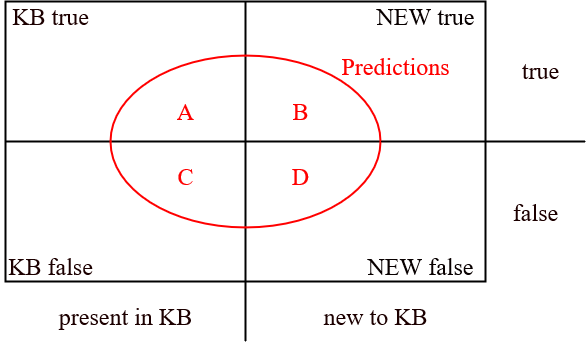
\includegraphics[width=10cm]{figures/kb_venn.png}
    \caption{KB prediction under incompleteness}
\end{figure}


\section{Rule-based machine learning}
Rule-based machine learning has as a goal to create rules that make new true predictions going beyond the data on which the rule was applied to. In contrast, other areas of machine learning focus on training a single model that can be applied to make a broad range of predictions. Conceptually the end result of rule-based machine learning is similar to a rule-based system.  Rule-based systems are often hand-crafted and require a knowledge expert to be curated, while rule-based machine learning requires no knowledge expert and rules are automatically created by the learning algorithm.

Classically, a rule is comprised of a condition and consequent, or a so-called "if-then" statement. \begin{center} \textbf{IF} \textit{'the condition is met'} \textbf{THEN} \textit{'the consequent holds'} \end{center}
The condition of the rule specifies attributes in the data on which the rule will be applied. If these attributes are present in this data, the condition is met. Once the condition for the rule is met, the attributes in the consequent should neccesarily also be met.

\begin{equation}
hasSibling(x, y) \Rightarrow hasSibling(y,x)
\label{example_rule_1}
\end{equation}
\begin{equation}
    hasSibling(x, y) \Rightarrow hasMother(x,z) \Rightarrow hasMOther(x, z)
    \label{example_rule_2}
\end{equation}
\begin{lstlisting}[caption={Simple example knowledge base},captionpos=b, label={simple_kb_example}]
<Ann> <hasMother> <Carol>
<Ann> <hasSibling> <Bob>
<Bob> <hasSibling> <Ann>
\end{lstlisting}
Consider the two rules and knowledge base given above. Under this knowledge base the antecedent of the first rule is satisfied by both triple 2 and 3. The resulting consequent of rule \ref{example_rule_1} is also present in the knowledge base. So the reflexivity of the $hasSibling$ predicate holds in this knowledge base. The antecendent of the second rule is satisfied by triples 1 and 2 in the knowledge base, but the resulting consquent would then be $hasMother(Bob, Carol)$. Since \texttt{<BoB> <hasMother> <Carol>} is not present in the knowledge base, rule \ref{example_rule_2} does not hold. If we know that this rule is reliable, we could for example extend the incomplete knowledge base with this triple.

Within rule-based machine learning there are many different approaches including learning classifier systems\cite{sigaud2007learning} and association rule mining\cite{agrawal1993mining}, the latter of which is the approach used in this thesis. Both approaches aim to create a set of rules to act as a model for a set of data. The association rule mining approach will now be explained further.


\subsection{Association Rule Mining}
Association rules \cite{agrawal1993mining} are types of "if-then" statements that describe frequent associations between items in a dataset containing \textit{transactions}. Association rule mining was originally proposed as a new method for finding relationships between sales items in stores. The idea of mining association rules over transactions has successfully been applied to many other scenarios \cite{altaf2017applications, lin2002efficient}. In the context of convenience store sales, each transaction can be thought of as a set of items that a customer has purchased. The rules are of the form $\{Sugar, Flour, Eggs\} \Rightarrow Butter$, meaning that a person who bought sugar, flour and eggs was likely to also purchase butter. The antecedent is some set of items in the dataset, while the consequent is an item often found in combination with the antecedent in the dataset.  So sugar, flour and eggs can be thought of as "associated with" butter. These original association rules are also not Horn rules over binary predicates, but is cited as a main inspiration for the AMIE approach used for experiments in this thesis.

\subsection{Significance and quality measurement}
The goal is to find formal rules that make true predictions that go beyond the explicit information in the knowledge base. For this some for of metrics are required in order to determine the suitability of a proposed rule.




Support and confidence were originally proposed as relevance and quality measurements for this type of rule mining, but as explained in \todo{PCA m8} this is not adequate when working with datasets in the form of knowledge graphs.

\[supp(\vec{B}\Rightarrow r(x, y)) :=  \# (x, y) : \exists z_1 , ...,z_m : \vec{B} \wedge r(x, y)\]

\[hc(\vec{B}\Rightarrow r(x, y)) := \frac{supp(\vec{B}\Rightarrow r(x, y)}{ \#(x', y'):r(x', y'))}\]

\[conf(\vec{B}\Rightarrow r(x, y)) := \frac{supp(\vec{B}\Rightarrow r(x, y)}{\#(x, y):\exists z_1 ,..., z_m : \vec{B}}\]

Partial completeness
\[\forall y' : r(x, y') \in KBtrue \cup NEWtrue \Rightarrow r(x, y') \in KBtrue\]

\[pcaconf(\vec{B}\Rightarrow r(x, y)) := \frac{supp(\vec{B}\Rightarrow r(x, y)}{\#(x, y):\exists z_1 ,..., z_m, y' : \vec{B} \wedge r(x, y')}\]


\subsection{AMIE3}

\iffalse 
\section{Web Ontology Language}
A widely used formal language for expressing ontologies is the \gls{owl}. In OWL "Daughters are female" could be formally expressed as:

\centerline{\textsf{SubClassOf(Daughter Female)}}
Information expressed in OWL can be used to draw new conclusions. For example if we know that an individual \emph{Amy} is a daughter, then we can makes the same conclusions as earlier about Amy being female. In OWL, the fact that Amy is in the class of females can be expressed as:

\centerline{\textsf{ClassAssertion(Female amy)}}
The task of reaching such conclusions is called reasoning and the type of conclusions that can be drawn is specified by the \gls{w3c}. It specifies the \emph{semantics} of OWL, but does not present algorithms for how to derive inferences in practice. Sound and complete reasoning in OWL is of high complexity \cite{Krotzsch2012}. Therefore, when the standard was updated to OWL 2 in 2009, it introduced restricted sublanguages to address this problem. These sublanguages restrict expressivity in order to simplify the reasoning task. One of these languages is OWL 2 QL, which is based on a \gls{dl} language called DL-Lite. OWL 2 QL is intended as a language to enable easier queries to databases. The ontology language we will use is DL-Lite$_{\mathcal{R}, horn}^{\exists}$, which is a member of the DL-Lite family.



\section{Description Logics}
\gls{dls} are a family of languages used in knowledge representation and reasoning. They are generally less expressive than \gls{fol}, but more expressive than \gls{pl}. The name \textit{description logic} represents two central aspects to this language group: \emph{description}, formal expression of knowledge, and  \emph{logic}, for it's logic-based semantics. DLs are used to represent domain knowledge in a well-structured and easily interpretable way. Domain knowledge is separated into two components in DL, a \emph{terminological} part, called a TBox, and an \emph{assertional} part, called an ABox. The TBox represents knowledge about the structure of the domain, while the ABox has knowledge about specific instances. For example the fact that \emph{cats are  mammals} would be a TBox statement, while \emph{Leo is a cat} would be an ABox statement, as here we are making an assertion about the individual Leo. The combination of a TBox and an ABox is called a \emph{knowledge base} (KB).
As the semantics of DLs are logic-based it is clear when a statement is \emph{entailed} by a KB. For instance the two examples given above entail that Leo is a mammal. More importantly, this reasoning task can be automated in a DL KB. Reasoning tasks are performed with respect to the entire KB, which gives this language great power, but also comes with a computational cost. Therefore an important area of research has been to find DLs that strike a balance between expressiveness and the computational complexity of reasoning.


The two main criteria for a reasoner is that it is decidable and tractable (always correctly completed in a time that is polynomial with respect to the size of the KB). The more operators one allows in a logic the more complicated the TBox becomes, and usually the complexity for reasoning in the language increases. See \href{http://www.cs.man.ac.uk/~ezolin/dl/}{\textbf{Complexity of reasoning in Description Logics}} for an interactive look at the complexity of different DLs \cite{zolin_2013}.

\section{The Resource Description Framework}

The Resource Description Framework (RDF) is a standard for representation and exchange of graph data introduced by \gls{w3c}. Semantic triples are the data types used in the RDF data model. A triple, as the name suggests, is a tuple of three elements. It has the form ( subject, predicate, object) and can therefore represent statements about semantic data, for example "Cats are mammals", or "Ann knows Bob". These RDF statements express relationships between two resources, these resources being the subject and the object, while the predicate encapsulates the nature of the relationship. The relationship is phrased in a directional way, and so set of RDF stamements can also be viewed as a directed graph. The graph represents these triple statements, where the predicate in the triple denotes the edge going from the subject to the object, both of which are vertices.

\begin{lstlisting}[caption={Example of RDF triple set written in informal pseudocode},label={RDF_triples_example}]
<Ann> <knows> <Bob>
<Ann> <is a> <person>
<Bob> <is a> <person>
<Ann> <owns> <Leo>
<Leo> <is a> <cat>
<cat> <is a> <mammal>
<Bob> <is scared of> <Leo>
\end{lstlisting}

\begin{figure}
\centering
    
\includegraphics[scale=0.3]{figures/RDF_triple}
    \caption{TODO Informal graph of the example triples from \ref{RDF_triples_example}}
    
    \label{fig:KGexample}
\end{figure}

With this type of data organisation one can for example query for a list of all people who own cats in the dataset.

\subsection{Resource Description Framework Schema}
RDF provides the abstract model for how to organize the data and sets standards for how data points relate to eachother and real-world entities. The RDF Schema (RDFS), on the other hand, is a \emph{vocabulary} in RDF that explains how nodes of a graph relate.

\section{Semantic Triples in Description Logics}
Semantic triples are 
\fi

\chapter{Related Works}

ONTOLOGICAL PATH FINDING
Chen, Y., Goldberg, S., Wang, D.Z., Johri, S.S.: Ontological Pathfinding. In: SIGMOD (2016) 
4. Chen, Y., Wang, D.Z., Goldberg, S.: ScaLeKB: Scalable Learning and Inference over Large Knowledge Bases. VLDB Journal 25(6) (2016)

\section{Section placeholder 1: works on knowledge graph embeddings}
A knowledge graph completion family that was not explored in this thesis is path-based reasoning methods. One of the first of these was the \textit{path ranking algorithm} (PRA) \cite{lao2011random}. This approach trains a binary classifier for each relation $r$ in the KG, that determines if given two entities $h$ and $t$ is they are connected via $r$. Path ranking algorithms struggle with sparseness in KGs \cite{ma2019elpkg}, and so there have been attempts at combining PRAs and embedding methods. An example of this is PTransE, which considers relation paths with multiple steps, and uses embedding methods similar to TransE to represent these paths \cite{lin2015modeling}. 

TODO: write about translation-based distance model vs semantic matching models

\section{Section placeholder 2: works on rule mining approaches}
Traditional rule mining methods find rules of quality by statistically evaluating support and confidence on candidate rules. AMIE and it's successors are part of this group, and have for a while been considered at the forefront of both efficiency and quality when it comes to mining first-order Horn rules from knowledge graphs. Exact statistical evaluation of rules is expensive, and so there have been approaches adopting embedding methods to score rules \cite{yang2014embedding. omran2018scalable, omran2019embedding}. The rule miner AnyBURL uses rule generation methods different from AMIE, where rules are generated by sampling paths in the KG \cite{meilicke2020reinforced}. These rules are evaluated with the same metrics as AMIE, but only approximated based on sampling in contrast to the exact evaluations in AMIE3. AnyBURL introduced the use of reinforcement learning to improve their sampling, leading to higher quality rules being found earlier in the search. A more recent approach to rule mining with reinforcement learning takes advantage of embedding information to achieve better performance and allows scalable mining of long rules \cite{chen2022rule}. This method also outperforms AMIE+, and the authors point out that the many optimizations made to AMIE+ (resulting in AMIE3) could be applied to any top-down rule mining methods, including theirs.  TODO: explain top down vs bottom up

https://arxiv.org/pdf/2004.04412.pdf

\section{Section placeholder 3: works that combine rule mining and KG embeddings}
Meilicke fuck yeah
https://openreview.net/forum?id=JQHqeGx6qFw

% Include more chapters as required.
%%=========================================
\renewcommand{\glossarypreamble}{\footnotesize}
\printglossary[style=super, type=\glsdefaulttype] \let\cleardoublepage\clearpage
\printglossary[style=super, type=\acronymtype]
% Include more appendices as required.
%%=========================================
\clearpage
\DeclareRobustCommand{\VAN}[3]{#3}
\addcontentsline{toc}{chapter}{Bibliography}
\bibliographystyle{generators/myplainnat}
\bibliography{generators/refs}
\appendix
\titleformat{\chapter}[display]
  {\normalfont\large\bfseries}% <- font for label "Appendix A", default \huge
  {\chaptertitlename\ \thechapter}
  {20pt}
  {\large}% <- font for title, default \Huge

\chapter{Results}


\begin{longtable}{llllll}
\textbf{child} & \textbf{father} & \textbf{mother} & \textbf{relative} & \textbf{sibling} & \textbf{spouse} \\ \hline
0.009  & -0.010 & -0.010 & -0.001   & 0.000   & 0.000  \\
0.002  & -0.002 & -0.002 & 0.000    & 0.000   & 0.000  \\
-0.001 & 0.001  & 0.002  & 0.001    & 0.000   & 0.000  \\
-0.005 & 0.005  & 0.005  & 0.000    & 0.000   & 0.000  \\
-0.012 & 0.012  & 0.012  & 0.001    & 0.000   & 0.001  \\
-0.007 & 0.008  & 0.007  & 0.001    & 0.000   & -0.001 \\
0.006  & -0.006 & -0.006 & -0.001   & 0.000   & 0.000  \\
-0.004 & 0.005  & 0.004  & 0.001    & 0.000   & 0.000  \\
0.003  & -0.002 & -0.002 & 0.001    & 0.000   & 0.000  \\
0.016  & -0.016 & -0.015 & 0.000    & 0.000   & 0.000  \\
-0.002 & 0.002  & 0.002  & 0.000    & 0.000   & 0.000  \\
-0.001 & 0.001  & 0.001  & 0.001    & 0.000   & 0.000  \\
0.006  & -0.005 & -0.006 & -0.001   & 0.000   & 0.000  \\
0.003  & -0.004 & -0.004 & 0.000    & 0.000   & 0.000  \\
-0.001 & 0.001  & 0.002  & -0.001   & 0.000   & 0.000  \\
-0.013 & 0.014  & 0.013  & -0.001   & 0.000   & 0.000  \\
0.008  & -0.008 & -0.008 & 0.000    & 0.000   & 0.000  \\
0.006  & -0.006 & -0.006 & -0.002   & 0.000   & 0.000  \\
-0.013 & 0.013  & 0.013  & 0.000    & 0.000   & 0.000  \\
-0.009 & 0.009  & 0.009  & 0.000    & 0.000   & 0.000  \\
-0.005 & 0.005  & 0.005  & 0.001    & 0.000   & 0.000  \\
-0.007 & 0.007  & 0.007  & 0.001    & 0.000   & 0.000  \\
0.001  & -0.001 & -0.001 & 0.000    & 0.000   & 0.001  \\
0.009  & -0.009 & -0.008 & -0.001   & 0.000   & 0.000  \\
-0.003 & 0.003  & 0.003  & 0.000    & 0.000   & 0.000  \\
0.003  & -0.003 & -0.003 & 0.000    & 0.000   & 0.000  \\
-0.014 & 0.014  & 0.014  & 0.001    & 0.000   & 0.001  \\
0.005  & -0.006 & -0.005 & 0.000    & 0.000   & 0.001  \\
-0.006 & 0.005  & 0.005  & 0.000    & 0.000   & 0.001  \\
0.000  & 0.000  & 0.000  & 0.001    & 0.000   & 0.000  \\
-0.003 & 0.003  & 0.003  & 0.000    & 0.000   & 0.000  \\
-0.003 & 0.003  & 0.004  & 0.001    & 0.000   & 0.000  \\
-0.009 & 0.009  & 0.009  & -0.001   & 0.000   & 0.000  \\
-0.011 & 0.011  & 0.010  & 0.001    & 0.000   & 0.000  \\
-0.001 & 0.001  & 0.001  & -0.001   & 0.000   & 0.000  \\
-0.009 & 0.009  & 0.008  & -0.001   & 0.000   & -0.001 \\
0.006  & -0.006 & -0.006 & -0.001   & 0.000   & 0.000  \\
-0.002 & 0.002  & 0.002  & 0.002    & 0.000   & 0.000  \\
0.002  & -0.002 & -0.002 & 0.000    & 0.000   & 0.000  \\
0.005  & -0.005 & -0.005 & -0.002   & 0.000   & 0.000  \\
-0.005 & 0.005  & 0.004  & 0.001    & 0.000   & 0.000  \\
0.007  & -0.007 & -0.006 & 0.001    & 0.000   & 0.000  \\
0.004  & -0.004 & -0.003 & 0.000    & 0.000   & 0.000  \\
0.005  & -0.006 & -0.006 & 0.001    & 0.000   & 0.000  \\
-0.005 & 0.006  & 0.005  & 0.001    & 0.000   & 0.001  \\
0.007  & -0.008 & -0.008 & -0.001   & 0.000   & 0.000  \\
0.005  & -0.005 & -0.004 & 0.000    & 0.000   & -0.001 \\
0.002  & -0.002 & -0.002 & -0.001   & 0.000   & 0.000  \\
0.003  & -0.003 & -0.002 & -0.001   & 0.000   & 0.001  \\
0.007  & -0.007 & -0.007 & 0.001    & 0.000   & 0.000  \\ \hline
\caption{TransE's 50-dimensional embedding vectors for the different relations in the family dataset, rounded to the third decimal. This table shows that the vectors for all relations are close to the zero-vector.}
\label{TransE_embedding_family}
\end{longtable}

\begin{longtable}{llllll}
\hline
\textbf{DRF} & \textbf{has\_part} & \textbf{hypernym} & \textbf{IH} & \textbf{MM} & \textbf{SDT} \\ \hline
0.000        & -0.002             & -0.003            & -0.004      & -0.027      & -0.028       \\
0.000        & 0.000              & 0.012             & 0.081       & -0.001      & 0.010        \\
0.000        & -0.003             & 0.007             & 0.010       & -0.012      & 0.009        \\
0.000        & -0.003             & 0.003             & -0.148      & -0.042      & 0.000        \\
0.000        & 0.017              & 0.003             & 0.005       & 0.002       & 0.007        \\
0.000        & -0.001             & 0.002             & 0.139       & -0.014      & 0.003        \\
0.000        & -0.002             & -0.002            & -0.115      & 0.031       & -0.006       \\
0.000        & -0.006             & 0.005             & 0.005       & -0.015      & 0.008        \\
0.000        & -0.001             & 0.001             & 0.150       & -0.021      & 0.010        \\
0.000        & -0.007             & -0.011            & 0.119       & 0.012       & 0.019        \\
0.000        & -0.004             & 0.013             & 0.118       & -0.019      & 0.012        \\
0.000        & -0.004             & -0.002            & -0.069      & 0.042       & -0.001       \\
0.000        & -0.002             & 0.002             & -0.165      & -0.025      & 0.002        \\
0.000        & 0.000              & -0.012            & -0.017      & 0.007       & -0.012       \\
0.000        & -0.018             & -0.002            & -0.111      & 0.008       & 0.015        \\
0.000        & 0.021              & 0.001             & 0.006       & 0.003       & -0.041       \\
0.000        & 0.001              & -0.015            & 0.005       & 0.043       & -0.026       \\
0.000        & -0.002             & 0.005             & -0.152      & -0.017      & -0.006       \\
0.000        & 0.002              & 0.002             & -0.082      & -0.002      & -0.009       \\
0.000        & -0.002             & 0.001             & 0.134       & -0.048      & 0.044        \\
0.000        & -0.001             & 0.007             & 0.142       & -0.003      & 0.016        \\
0.000        & -0.001             & -0.001            & -0.134      & -0.060      & -0.009       \\
0.000        & 0.018              & -0.003            & -0.142      & -0.020      & -0.016       \\
0.000        & 0.002              & -0.008            & -0.084      & 0.010       & -0.030       \\
0.000        & -0.004             & 0.009             & -0.062      & -0.007      & -0.019       \\
0.000        & 0.005              & 0.005             & 0.067       & 0.000       & 0.011        \\
0.000        & -0.003             & 0.005             & 0.113       & -0.009      & 0.028        \\
0.000        & 0.002              & -0.005            & 0.002       & -0.038      & -0.010       \\
0.000        & 0.007              & 0.001             & -0.127      & 0.000       & -0.010       \\
0.000        & -0.002             & 0.000             & 0.036       & -0.007      & 0.013        \\
0.001        & -0.005             & 0.002             & 0.002       & 0.009       & -0.010       \\
0.000        & -0.004             & 0.004             & -0.075      & -0.045      & 0.017        \\
-0.001       & 0.016              & 0.001             & 0.110       & 0.018       & -0.024       \\
0.000        & 0.009              & 0.000             & 0.156       & -0.002      & -0.020       \\
0.001        & 0.000              & 0.007             & 0.023       & -0.043      & -0.001       \\
0.000        & -0.002             & -0.003            & -0.103      & 0.001       & 0.000        \\
0.000        & -0.008             & 0.007             & 0.167       & -0.005      & 0.019        \\
0.000        & 0.000              & -0.017            & 0.021       & 0.012       & -0.020       \\
0.000        & -0.007             & -0.003            & -0.001      & 0.025       & -0.002       \\
0.000        & -0.008             & -0.006            & 0.029       & 0.047       & 0.006        \\
-0.001       & 0.002              & 0.000             & -0.001      & 0.047       & -0.004       \\
0.000        & -0.002             & 0.014             & 0.139       & -0.036      & 0.005        \\
0.000        & 0.001              & 0.010             & 0.010       & -0.056      & 0.003        \\
0.000        & -0.001             & 0.001             & -0.005      & 0.000       & 0.019        \\
0.000        & -0.002             & -0.001            & -0.128      & 0.005       & 0.007        \\
0.000        & -0.001             & 0.002             & 0.131       & 0.001       & -0.002       \\
0.000        & -0.004             & 0.011             & 0.137       & -0.008      & 0.024        \\
0.000        & 0.005              & -0.002            & -0.092      & -0.045      & -0.006       \\
0.000        & 0.001              & 0.011             & -0.058      & -0.005      & -0.023       \\
0.000        & 0.004              & -0.013            & -0.041      & 0.021       & -0.046      \\ \hline
\caption{TransE's 50-dimensional embedding vectors for the different relations in the WN18RR dataset, rounded to the third decimal. This table shows that the vectors for all relations are close to the zero-vector. \textbf{DRF} = \textit{derivationally\_related\_form}, \textbf{IH} = \textit{instance\_hypernym}, \textbf{MM} = \textit{member\_meronym} and \textbf{SDT} = \textit{synset\_domain\_topic of}.}
\label{TransE_embedding_WN18RR}
\end{longtable}

\begin{figure}[htbp]
\centering
    \centering
    \includesvg[inkscapelatex=false,width=0.6\textwidth,keepaspectratio]{figures/appendix/all_sets.svg}
    \caption[Dist. of all sets of mined rules.]{Distribution of all mined rule sets. Each rule set is labeled with the entity selection strategy, embedding model and rank cutoff that was used for that particular KG extension. As mentioned in section \ref{TransE_sucks} can see that when the KGs are extended using TransE the number of new rules that are mined increases drastically.}
    \label{all_sets}
\end{figure}


\begin{figure}[htbp]
\centering
    \centering
    \includesvg[inkscapelatex=false,width=0.75\textwidth,keepaspectratio]{figures/appendix/all_sets_w_out_TransE.svg}
    \caption[Dist. of all sets of mined rules, excluding TransE.]{Distribution of all mined rule sets, excluding the sets mined from KGs extended using TransE. Each rule set is labeled with the entity selection strategy, embedding model and rank cutoff that was used for that particular KG extension. We can observe that no new rules are mined when the RandomBaseline was used to extend the KGs.}
    \label{all_sets_w_out_TransE}
\end{figure}
\iffalse
\begin{table}
\begin{tabular}{lrr}
\toprule
                                                                                                      Rule &  Frequencies &  PCA Confidence \\
\midrule
                            y  DRF  x   $\Rightarrow$ x  DRF  y &           48 &        1.000000 \\
                   x  \_hypernym  z  z  SDTO  y   $\Rightarrow$ x  SDTO  y &           36 &        0.828871 \\
                   z  \_hypernym  x  z  SDTO  y   $\Rightarrow$ x  SDTO  y &           34 &        0.726667 \\
                   x  \_has\_part  z  z  SDTO  y   $\Rightarrow$ x  SDTO  y &           24 &        0.809524 \\
          x  IH  z  z  SDTO  y   $\Rightarrow$ x  SDTO  y &           24 &        0.886525 \\
x  DRF  z  z  SDTO  y   $\Rightarrow$ x  SDTO  y &           24 &        0.492857 \\
z  DRF  x  z  SDTO  y   $\Rightarrow$ x  SDTO  y &           24 &        0.492857 \\
                   z  \_has\_part  x  z  SDTO  y   $\Rightarrow$ x  SDTO  y &           24 &        0.771739 \\
                                               x  \_has\_part  z  y  \_hypernym  z   $\Rightarrow$ x  \_has\_part  y &           21 &        0.104016 \\
                                      x  \_has\_part  z  y  IH  z   $\Rightarrow$ x  \_has\_part  y &           19 &        0.532544 \\
\bottomrule
\end{tabular}
\caption{Rules mined from the original WN18RR KG, with their corresponding PCA confidences and how many times they were mined from the 48 extensions. DRF = ``\textit{derivationally related form}", STDO = ``\textit{synset domain topic of}" and IH = ``\textit{instance hypernym}".}
\label{wn18rr_original_rules_table_frequencies}
\end{table}

\begin{table}
\begin{tabular}{lrr}
\toprule
                                                                                                      Rule &  Frequencies &  PCA Confidence \\
\midrule
                            y  DRF  x   $\Rightarrow$ x  DRF  y &           48 &        1.000000 \\
          x  IH  z  z  SDTO  y   $\Rightarrow$ x  SDTO  y &           24 &        0.886525 \\
                   x  \_hypernym  z  z  SDTO  y   $\Rightarrow$ x  SDTO  y &           36 &        0.828871 \\
                   x  \_has\_part  z  z  SDTO  y   $\Rightarrow$ x  SDTO  y &           24 &        0.809524 \\
                   z  \_has\_part  x  z  SDTO  y   $\Rightarrow$ x  SDTO  y &           24 &        0.771739 \\
                   z  \_hypernym  x  z  SDTO  y   $\Rightarrow$ x  SDTO  y &           34 &        0.726667 \\
                                      x  \_has\_part  z  y  IH  z   $\Rightarrow$ x  \_has\_part  y &           19 &        0.532544 \\
x  DRF  z  z  SDTO  y   $\Rightarrow$ x  SDTO  y &           24 &        0.492857 \\
z  DRF  x  z  SDTO  y   $\Rightarrow$ x  SDTO  y &           24 &        0.492857 \\
                                               x  \_has\_part  z  y  \_hypernym  z   $\Rightarrow$ x  \_has\_part  y &           21 &        0.104016 \\
\bottomrule
\end{tabular}
https://www.overleaf.com/project/6065c0290955e6097131b67b\caption{Rules mined from the original WN18RR KG, with their corresponding PCA confidences and how many times they were mined from the 48 extensions. DRF = ``\textit{derivationally related form}", STDO = ``\textit{synset domain topic of}" and IH = ``\textit{instance hypernym}".}
\label{wn18rr_original_rules_table_PCA}
\end{table}

\begin{longtable}{lrr}
\toprule
                                                    Rule &  Frequencies &  PCA Confidence \\
\midrule
                  relative(y, x)   $\Rightarrow$ relative(x, y) &           48 &        0.846306 \\
      mother(x, z) $\wedge$ spouse(z, y)   $\Rightarrow$ father(x, y) &           48 &        0.872686 \\
       child(z, x) $\wedge$ spouse(z, y)   $\Rightarrow$ father(x, y) &           48 &        0.350117 \\
      mother(z, x) $\wedge$ sibling(y, z)   $\Rightarrow$ child(x, y) &           48 &        0.704016 \\
        child(x, z) $\wedge$ child(y, z)   $\Rightarrow$ spouse(x, y) &           48 &        0.471973 \\
      child(y, z) $\wedge$ sibling(x, z)   $\Rightarrow$ father(x, y) &           48 &        0.584069 \\
      mother(z, x) $\wedge$ sibling(z, y)   $\Rightarrow$ child(x, y) &           48 &        0.703385 \\
      child(y, z) $\wedge$ sibling(z, x)   $\Rightarrow$ father(x, y) &           48 &        0.583590 \\
       child(z, x) $\wedge$ spouse(y, z)   $\Rightarrow$ father(x, y) &           48 &        0.351479 \\
       child(x, z) $\wedge$ father(z, y)   $\Rightarrow$ spouse(x, y) &           48 &        0.471666 \\
      mother(x, z) $\wedge$ spouse(y, z)   $\Rightarrow$ father(x, y) &           48 &        0.867655 \\
       child(z, x) $\wedge$ spouse(z, y)   $\Rightarrow$ mother(x, y) &           48 &        0.386296 \\
       child(y, z) $\wedge$ mother(z, x)   $\Rightarrow$ spouse(x, y) &           48 &        0.480628 \\
       child(y, z) $\wedge$ father(z, x)   $\Rightarrow$ spouse(x, y) &           48 &        0.469716 \\
      child(y, z) $\wedge$ sibling(z, x)   $\Rightarrow$ mother(x, y) &           48 &        0.422363 \\
      father(x, z) $\wedge$ spouse(y, z)   $\Rightarrow$ mother(x, y) &           48 &        0.701812 \\
     mother(z, y) $\wedge$ sibling(z, x)   $\Rightarrow$ mother(x, y) &           48 &        0.787401 \\
     mother(z, y) $\wedge$ sibling(x, z)   $\Rightarrow$ mother(x, y) &           48 &        0.787816 \\
       child(z, x) $\wedge$ spouse(y, z)   $\Rightarrow$ mother(x, y) &           48 &        0.382227 \\
      child(y, z) $\wedge$ sibling(x, z)   $\Rightarrow$ mother(x, y) &           48 &        0.422559 \\
       child(x, z) $\wedge$ mother(z, y)   $\Rightarrow$ spouse(x, y) &           48 &        0.477785 \\
      father(x, z) $\wedge$ spouse(z, y)   $\Rightarrow$ mother(x, y) &           48 &        0.708957 \\
       mother(y, z) $\wedge$ spouse(x, z)   $\Rightarrow$ child(x, y) &           48 &        0.838288 \\
     father(z, y) $\wedge$ sibling(x, z)   $\Rightarrow$ father(x, y) &           48 &        0.961023 \\
      father(z, x) $\wedge$ sibling(z, y)   $\Rightarrow$ child(x, y) &           48 &        0.954328 \\
        child(z, y) $\wedge$ spouse(x, z)   $\Rightarrow$ child(x, y) &           48 &        0.688723 \\
       child(z, x) $\wedge$ child(z, y)   $\Rightarrow$ sibling(x, y) &           48 &        0.664745 \\
   sibling(z, x) $\wedge$ sibling(z, y)   $\Rightarrow$ sibling(x, y) &           48 &        0.564657 \\
     father(x, z) $\wedge$ father(y, z)   $\Rightarrow$ sibling(x, y) &           48 &        0.658865 \\
   sibling(z, y) $\wedge$ sibling(x, z)   $\Rightarrow$ sibling(x, y) &           48 &        0.588151 \\
   sibling(x, z) $\wedge$ sibling(y, z)   $\Rightarrow$ sibling(x, y) &           48 &        0.590059 \\
   sibling(z, x) $\wedge$ sibling(y, z)   $\Rightarrow$ sibling(x, y) &           48 &        0.584857 \\
      child(z, y) $\wedge$ father(x, z)   $\Rightarrow$ sibling(x, y) &           48 &        0.662206 \\
      child(z, x) $\wedge$ father(y, z)   $\Rightarrow$ sibling(x, y) &           48 &        0.668446 \\
       child(x, z) $\wedge$ sibling(z, y)   $\Rightarrow$ child(x, y) &           48 &        0.850519 \\
       father(y, z) $\wedge$ spouse(x, z)   $\Rightarrow$ child(x, y) &           48 &        0.588257 \\
       child(x, z) $\wedge$ sibling(y, z)   $\Rightarrow$ child(x, y) &           48 &        0.851012 \\
     father(z, y) $\wedge$ sibling(z, x)   $\Rightarrow$ father(x, y) &           48 &        0.961199 \\
     mother(x, z) $\wedge$ mother(y, z)   $\Rightarrow$ sibling(x, y) &           48 &        0.707149 \\
       father(y, z) $\wedge$ spouse(z, x)   $\Rightarrow$ child(x, y) &           48 &        0.588533 \\
      child(z, y) $\wedge$ mother(x, z)   $\Rightarrow$ sibling(x, y) &           48 &        0.709139 \\
      father(z, x) $\wedge$ sibling(y, z)   $\Rightarrow$ child(x, y) &           48 &        0.954603 \\
      child(z, x) $\wedge$ mother(y, z)   $\Rightarrow$ sibling(x, y) &           48 &        0.709805 \\
        child(z, y) $\wedge$ spouse(z, x)   $\Rightarrow$ child(x, y) &           48 &        0.687653 \\
       mother(y, z) $\wedge$ spouse(z, x)   $\Rightarrow$ child(x, y) &           48 &        0.839947 \\
                       child(y, x)   $\Rightarrow$ mother(x, y) &           48 &        0.535350 \\
      father(z, y) $\wedge$ mother(z, x)   $\Rightarrow$ spouse(x, y) &           48 &        0.967952 \\
      father(z, x) $\wedge$ mother(z, y)   $\Rightarrow$ spouse(x, y) &           48 &        0.953170 \\
                      spouse(y, x)   $\Rightarrow$ spouse(x, y) &           48 &        0.992355 \\
                       father(y, x)   $\Rightarrow$ child(x, y) &           48 &        0.998071 \\
                    sibling(y, x)   $\Rightarrow$ sibling(x, y) &           48 &        0.989634 \\
                       mother(y, x)   $\Rightarrow$ child(x, y) &           48 &        0.991906 \\
                       child(y, x)   $\Rightarrow$ father(x, y) &           48 &        0.769746 \\
 relative(z, x) $\wedge$ sibling(y, z)   $\Rightarrow$ relative(x, y) &           40 &        0.348765 \\
 relative(z, x) $\wedge$ sibling(z, y)   $\Rightarrow$ relative(x, y) &           40 &        0.351014 \\
 relative(x, z) $\wedge$ sibling(z, y)   $\Rightarrow$ relative(x, y) &           40 &        0.483459 \\
 relative(x, z) $\wedge$ sibling(y, z)   $\Rightarrow$ relative(x, y) &           40 &        0.484528 \\
 relative(z, y) $\wedge$ sibling(z, x)   $\Rightarrow$ relative(x, y) &           39 &        0.126881 \\
 relative(z, y) $\wedge$ sibling(x, z)   $\Rightarrow$ relative(x, y) &           39 &        0.127978 \\
 relative(y, z) $\wedge$ sibling(x, z)   $\Rightarrow$ relative(x, y) &           38 &        0.120360 \\
 relative(y, z) $\wedge$ sibling(z, x)   $\Rightarrow$ relative(x, y) &           38 &        0.120448 \\
   child(y, z) $\wedge$ relative(z, x)   $\Rightarrow$ relative(x, y) &           37 &        0.273356 \\
  father(z, y) $\wedge$ relative(x, z)   $\Rightarrow$ relative(x, y) &           37 &        0.372340 \\
  relative(x, z) $\wedge$ spouse(z, y)   $\Rightarrow$ relative(x, y) &           37 &        0.305043 \\
  relative(x, z) $\wedge$ spouse(y, z)   $\Rightarrow$ relative(x, y) &           37 &        0.305043 \\
  father(y, z) $\wedge$ relative(x, z)   $\Rightarrow$ relative(x, y) &           37 &        0.378085 \\
   child(z, y) $\wedge$ relative(z, x)   $\Rightarrow$ relative(x, y) &           37 &        0.275454 \\
   child(y, z) $\wedge$ relative(x, z)   $\Rightarrow$ relative(x, y) &           37 &        0.343180 \\
  father(y, z) $\wedge$ relative(z, x)   $\Rightarrow$ relative(x, y) &           37 &        0.294304 \\
  father(z, y) $\wedge$ relative(z, x)   $\Rightarrow$ relative(x, y) &           37 &        0.301061 \\
   child(z, y) $\wedge$ relative(x, z)   $\Rightarrow$ relative(x, y) &           37 &        0.364472 \\
  mother(y, z) $\wedge$ relative(x, z)   $\Rightarrow$ relative(x, y) &           36 &        0.350490 \\
  relative(z, x) $\wedge$ spouse(y, z)   $\Rightarrow$ relative(x, y) &           35 &        0.206044 \\
  mother(y, z) $\wedge$ relative(z, x)   $\Rightarrow$ relative(x, y) &           33 &        0.241645 \\
  mother(z, y) $\wedge$ relative(x, z)   $\Rightarrow$ relative(x, y) &           33 &        0.283544 \\
  father(z, x) $\wedge$ relative(y, z)   $\Rightarrow$ relative(x, y) &           33 &        0.179144 \\
   child(x, z) $\wedge$ relative(y, z)   $\Rightarrow$ relative(x, y) &           32 &        0.148287 \\
  relative(z, x) $\wedge$ spouse(z, y)   $\Rightarrow$ relative(x, y) &           32 &        0.205761 \\
   child(x, z) $\wedge$ relative(z, y)   $\Rightarrow$ relative(x, y) &           31 &        0.123643 \\
    father(z, x) $\wedge$ father(y, z)   $\Rightarrow$ relative(x, y) &           30 &        0.196078 \\
  mother(z, y) $\wedge$ relative(z, x)   $\Rightarrow$ relative(x, y) &           30 &        0.224490 \\
  father(z, x) $\wedge$ relative(z, y)   $\Rightarrow$ relative(x, y) &           30 &        0.140871 \\
relative(z, y) $\wedge$ relative(x, z)   $\Rightarrow$ relative(x, y) &           29 &        0.100440 \\
     child(x, z) $\wedge$ father(y, z)   $\Rightarrow$ relative(x, y) &           27 &        0.153584 \\
     child(z, y) $\wedge$ father(z, x)   $\Rightarrow$ relative(x, y) &           26 &        0.166667 \\
      child(z, y) $\wedge$ child(x, z)   $\Rightarrow$ relative(x, y) &           25 &        0.130759 \\
    father(z, x) $\wedge$ spouse(y, z)   $\Rightarrow$ relative(x, y) &           21 &        0.124101 \\
  mother(x, z) $\wedge$ relative(y, z)   $\Rightarrow$ relative(x, y) &           21 &        0.104492 \\
  mother(z, x) $\wedge$ relative(y, z)   $\Rightarrow$ relative(x, y) &           18 &        0.101064 \\
    father(z, x) $\wedge$ spouse(z, y)   $\Rightarrow$ relative(x, y) &           17 &        0.122083 \\
    father(z, y) $\wedge$ father(x, z)   $\Rightarrow$ relative(x, y) &           16 &        0.108774 \\
     child(x, z) $\wedge$ spouse(y, z)   $\Rightarrow$ relative(x, y) &           13 &        0.102020 \\
     child(x, z) $\wedge$ spouse(z, y)   $\Rightarrow$ relative(x, y) &           13 &        0.102020 \\
   father(x, z) $\wedge$ sibling(z, y)   $\Rightarrow$ relative(x, y) &           10 &        0.100971 \\
\bottomrule
\caption{Rules mined from the original family KG, with their corresponding PCA confidences and how many times they were mined from the 48 extensions. Note that all rules with the $relative$ predicate in the consequent have lower PCA confidence and were mined less frequently.}
\label{family_original_rules_table_frequencies}
\end{longtable}
\fi


\newpage
\begin{longtable}{lrr}
\toprule
                                                    Rule &  Frequencies &  PCA Confidence \\
\midrule
                       father(y, x)   $\Rightarrow$ child(x, y) &           48 &        0.998071 \\
                      spouse(y, x)   $\Rightarrow$ spouse(x, y) &           48 &        0.992355 \\
                       mother(y, x)   $\Rightarrow$ child(x, y) &           48 &        0.991906 \\
                    sibling(y, x)   $\Rightarrow$ sibling(x, y) &           48 &        0.989634 \\
      father(z, y) $\wedge$ mother(z, x)   $\Rightarrow$ spouse(x, y) &           48 &        0.967952 \\
     father(z, y) $\wedge$ sibling(z, x)   $\Rightarrow$ father(x, y) &           48 &        0.961199 \\
     father(z, y) $\wedge$ sibling(x, z)   $\Rightarrow$ father(x, y) &           48 &        0.961023 \\
      father(z, x) $\wedge$ sibling(y, z)   $\Rightarrow$ child(x, y) &           48 &        0.954603 \\
      father(z, x) $\wedge$ sibling(z, y)   $\Rightarrow$ child(x, y) &           48 &        0.954328 \\
      father(z, x) $\wedge$ mother(z, y)   $\Rightarrow$ spouse(x, y) &           48 &        0.953170 \\
      mother(x, z) $\wedge$ spouse(z, y)   $\Rightarrow$ father(x, y) &           48 &        0.872686 \\
      mother(x, z) $\wedge$ spouse(y, z)   $\Rightarrow$ father(x, y) &           48 &        0.867655 \\
       child(x, z) $\wedge$ sibling(y, z)   $\Rightarrow$ child(x, y) &           48 &        0.851012 \\
       child(x, z) $\wedge$ sibling(z, y)   $\Rightarrow$ child(x, y) &           48 &        0.850519 \\
                  relative(y, x)   $\Rightarrow$ relative(x, y) &           48 &        0.846306 \\
       mother(y, z) $\wedge$ spouse(z, x)   $\Rightarrow$ child(x, y) &           48 &        0.839947 \\
       mother(y, z) $\wedge$ spouse(x, z)   $\Rightarrow$ child(x, y) &           48 &        0.838288 \\
     mother(z, y) $\wedge$ sibling(x, z)   $\Rightarrow$ mother(x, y) &           48 &        0.787816 \\
     mother(z, y) $\wedge$ sibling(z, x)   $\Rightarrow$ mother(x, y) &           48 &        0.787401 \\
                       child(y, x)   $\Rightarrow$ father(x, y) &           48 &        0.769746 \\
      child(z, x) $\wedge$ mother(y, z)   $\Rightarrow$ sibling(x, y) &           48 &        0.709805 \\
      child(z, y) $\wedge$ mother(x, z)   $\Rightarrow$ sibling(x, y) &           48 &        0.709139 \\
      father(x, z) $\wedge$ spouse(z, y)   $\Rightarrow$ mother(x, y) &           48 &        0.708957 \\
     mother(x, z) $\wedge$ mother(y, z)   $\Rightarrow$ sibling(x, y) &           48 &        0.707149 \\
      mother(z, x) $\wedge$ sibling(y, z)   $\Rightarrow$ child(x, y) &           48 &        0.704016 \\
      mother(z, x) $\wedge$ sibling(z, y)   $\Rightarrow$ child(x, y) &           48 &        0.703385 \\
      father(x, z) $\wedge$ spouse(y, z)   $\Rightarrow$ mother(x, y) &           48 &        0.701812 \\
        child(z, y) $\wedge$ spouse(x, z)   $\Rightarrow$ child(x, y) &           48 &        0.688723 \\
        child(z, y) $\wedge$ spouse(z, x)   $\Rightarrow$ child(x, y) &           48 &        0.687653 \\
      child(z, x) $\wedge$ father(y, z)   $\Rightarrow$ sibling(x, y) &           48 &        0.668446 \\
       child(z, x) $\wedge$ child(z, y)   $\Rightarrow$ sibling(x, y) &           48 &        0.664745 \\
      child(z, y) $\wedge$ father(x, z)   $\Rightarrow$ sibling(x, y) &           48 &        0.662206 \\
     father(x, z) $\wedge$ father(y, z)   $\Rightarrow$ sibling(x, y) &           48 &        0.658865 \\
   sibling(x, z) $\wedge$ sibling(y, z)   $\Rightarrow$ sibling(x, y) &           48 &        0.590059 \\
       father(y, z) $\wedge$ spouse(z, x)   $\Rightarrow$ child(x, y) &           48 &        0.588533 \\
       father(y, z) $\wedge$ spouse(x, z)   $\Rightarrow$ child(x, y) &           48 &        0.588257 \\
   sibling(z, y) $\wedge$ sibling(x, z)   $\Rightarrow$ sibling(x, y) &           48 &        0.588151 \\
   sibling(z, x) $\wedge$ sibling(y, z)   $\Rightarrow$ sibling(x, y) &           48 &        0.584857 \\
      child(y, z) $\wedge$ sibling(x, z)   $\Rightarrow$ father(x, y) &           48 &        0.584069 \\
      child(y, z) $\wedge$ sibling(z, x)   $\Rightarrow$ father(x, y) &           48 &        0.583590 \\
   sibling(z, x) $\wedge$ sibling(z, y)   $\Rightarrow$ sibling(x, y) &           48 &        0.564657 \\
                       child(y, x)   $\Rightarrow$ mother(x, y) &           48 &        0.535350 \\
 relative(x, z) $\wedge$ sibling(y, z)   $\Rightarrow$ relative(x, y) &           40 &        0.484528 \\
 relative(x, z) $\wedge$ sibling(z, y)   $\Rightarrow$ relative(x, y) &           40 &        0.483459 \\
       child(y, z) $\wedge$ mother(z, x)   $\Rightarrow$ spouse(x, y) &           48 &        0.480628 \\
       child(x, z) $\wedge$ mother(z, y)   $\Rightarrow$ spouse(x, y) &           48 &        0.477785 \\
        child(x, z) $\wedge$ child(y, z)   $\Rightarrow$ spouse(x, y) &           48 &        0.471973 \\
       child(x, z) $\wedge$ father(z, y)   $\Rightarrow$ spouse(x, y) &           48 &        0.471666 \\
       child(y, z) $\wedge$ father(z, x)   $\Rightarrow$ spouse(x, y) &           48 &        0.469716 \\
      child(y, z) $\wedge$ sibling(x, z)   $\Rightarrow$ mother(x, y) &           48 &        0.422559 \\
      child(y, z) $\wedge$ sibling(z, x)   $\Rightarrow$ mother(x, y) &           48 &        0.422363 \\
       child(z, x) $\wedge$ spouse(z, y)   $\Rightarrow$ mother(x, y) &           48 &        0.386296 \\
       child(z, x) $\wedge$ spouse(y, z)   $\Rightarrow$ mother(x, y) &           48 &        0.382227 \\
  father(y, z) $\wedge$ relative(x, z)   $\Rightarrow$ relative(x, y) &           37 &        0.378085 \\
  father(z, y) $\wedge$ relative(x, z)   $\Rightarrow$ relative(x, y) &           37 &        0.372340 \\
   child(z, y) $\wedge$ relative(x, z)   $\Rightarrow$ relative(x, y) &           37 &        0.364472 \\
       child(z, x) $\wedge$ spouse(y, z)   $\Rightarrow$ father(x, y) &           48 &        0.351479 \\
 relative(z, x) $\wedge$ sibling(z, y)   $\Rightarrow$ relative(x, y) &           40 &        0.351014 \\
  mother(y, z) $\wedge$ relative(x, z)   $\Rightarrow$ relative(x, y) &           36 &        0.350490 \\
       child(z, x) $\wedge$ spouse(z, y)   $\Rightarrow$ father(x, y) &           48 &        0.350117 \\
 relative(z, x) $\wedge$ sibling(y, z)   $\Rightarrow$ relative(x, y) &           40 &        0.348765 \\
   child(y, z) $\wedge$ relative(x, z)   $\Rightarrow$ relative(x, y) &           37 &        0.343180 \\
  relative(x, z) $\wedge$ spouse(z, y)   $\Rightarrow$ relative(x, y) &           37 &        0.305043 \\
  relative(x, z) $\wedge$ spouse(y, z)   $\Rightarrow$ relative(x, y) &           37 &        0.305043 \\
  father(z, y) $\wedge$ relative(z, x)   $\Rightarrow$ relative(x, y) &           37 &        0.301061 \\
  father(y, z) $\wedge$ relative(z, x)   $\Rightarrow$ relative(x, y) &           37 &        0.294304 \\
  mother(z, y) $\wedge$ relative(x, z)   $\Rightarrow$ relative(x, y) &           33 &        0.283544 \\
   child(z, y) $\wedge$ relative(z, x)   $\Rightarrow$ relative(x, y) &           37 &        0.275454 \\
   child(y, z) $\wedge$ relative(z, x)   $\Rightarrow$ relative(x, y) &           37 &        0.273356 \\
  mother(y, z) $\wedge$ relative(z, x)   $\Rightarrow$ relative(x, y) &           33 &        0.241645 \\
  mother(z, y) $\wedge$ relative(z, x)   $\Rightarrow$ relative(x, y) &           30 &        0.224490 \\
  relative(z, x) $\wedge$ spouse(y, z)   $\Rightarrow$ relative(x, y) &           35 &        0.206044 \\
  relative(z, x) $\wedge$ spouse(z, y)   $\Rightarrow$ relative(x, y) &           32 &        0.205761 \\
    father(z, x) $\wedge$ father(y, z)   $\Rightarrow$ relative(x, y) &           30 &        0.196078 \\
  father(z, x) $\wedge$ relative(y, z)   $\Rightarrow$ relative(x, y) &           33 &        0.179144 \\
     child(z, y) $\wedge$ father(z, x)   $\Rightarrow$ relative(x, y) &           26 &        0.166667 \\
     child(x, z) $\wedge$ father(y, z)   $\Rightarrow$ relative(x, y) &           27 &        0.153584 \\
   child(x, z) $\wedge$ relative(y, z)   $\Rightarrow$ relative(x, y) &           32 &        0.148287 \\
  father(z, x) $\wedge$ relative(z, y)   $\Rightarrow$ relative(x, y) &           30 &        0.140871 \\
      child(z, y) $\wedge$ child(x, z)   $\Rightarrow$ relative(x, y) &           25 &        0.130759 \\
 relative(z, y) $\wedge$ sibling(x, z)   $\Rightarrow$ relative(x, y) &           39 &        0.127978 \\
 relative(z, y) $\wedge$ sibling(z, x)   $\Rightarrow$ relative(x, y) &           39 &        0.126881 \\
    father(z, x) $\wedge$ spouse(y, z)   $\Rightarrow$ relative(x, y) &           21 &        0.124101 \\
   child(x, z) $\wedge$ relative(z, y)   $\Rightarrow$ relative(x, y) &           31 &        0.123643 \\
    father(z, x) $\wedge$ spouse(z, y)   $\Rightarrow$ relative(x, y) &           17 &        0.122083 \\
 relative(y, z) $\wedge$ sibling(z, x)   $\Rightarrow$ relative(x, y) &           38 &        0.120448 \\
 relative(y, z) $\wedge$ sibling(x, z)   $\Rightarrow$ relative(x, y) &           38 &        0.120360 \\
    father(z, y) $\wedge$ father(x, z)   $\Rightarrow$ relative(x, y) &           16 &        0.108774 \\
  mother(x, z) $\wedge$ relative(y, z)   $\Rightarrow$ relative(x, y) &           21 &        0.104492 \\
     child(x, z) $\wedge$ spouse(y, z)   $\Rightarrow$ relative(x, y) &           13 &        0.102020 \\
     child(x, z) $\wedge$ spouse(z, y)   $\Rightarrow$ relative(x, y) &           13 &        0.102020 \\
  mother(z, x) $\wedge$ relative(y, z)   $\Rightarrow$ relative(x, y) &           18 &        0.101064 \\
   father(x, z) $\wedge$ sibling(z, y)   $\Rightarrow$ relative(x, y) &           10 &        0.100971 \\
relative(z, y) $\wedge$ relative(x, z)   $\Rightarrow$ relative(x, y) &           29 &        0.100440 \\
\bottomrule
\caption[Rules mined from the original family KG]{Rules mined from the original family KG, with their corresponding PCA confidences and how many times they were mined from the 48 extensions. Note that all rules with the $relative$ predicate in the consequent have lower PCA confidence and were mined less frequently.}
\label{family_original_rules_table_PCA}
\end{longtable}


\section{Propositional logic}
\label{propositional_logic}
Propositional logic (PL) is a branch of logic that deals with statements, or ``propositions", that can be either true or false. Propositions can be combined using boolean operators, for example ``and" $\wedge$ (conjunction) and ``or" $\vee$ (disjunction). Atomic propositions are propositions without operators, and are also called \textit{literals}. Literals are boolean variables $v$ or their negation $\neg v$. For example, two literals $v_1, v_2$ can be combined to one proposition $P$ with the ``or" operator:
\[P = \neg v_1 \vee v_2\]
Now $P$ evaluates to true if $v_1$ is evaluated to false or if $v_2$ is evaluated to true. The proposition $P$ will only evaluate to false if $v_1$ is true \textit{and} $v_2$ is false. A \textit{clause} is a disjunction of literals, so $P$ is a clause. The proposition $P$ is also considered a \textit{Horn clause}, which is a clause where at most one literal is not negated. 

The implication operator is denoted by $\rightarrow$, and can be thought of as an "if-then" operator. The proposition $v_1 \rightarrow v_2$ can be read as ``\textit{if} $v_1$\textit{ is true, then }$v_2$ \textit{is true}". The statement is thus only falsified if $v_1$ is true and $v_2$ is false. If $v_2$ is true then it does not matter what $v_1$ evaluates to, and similarly if $v_1$ is false then it does not matter what $v_2$ evaluates to. If we compare this to the circumstances under which $P$ evaluated to true and false we also see that $P = v_1 \rightarrow v_2 = \neg v_1 \vee v_2$. 
Thus, in a Horn clauses can be treated as rules, where all the negated literals are in the antecedent (on the left side of the implication arrow) and the single non-negated literal is the consequent (on the right side of the implication arrow). For example the proposition \[Q = v_1 \wedge v_3 \wedge v_4\rightarrow v_2 = \neg v_1 \vee \neg v_3 \vee \neg v_4\vee v_2\] is also a Horn clause. The rule mining algorithm AMIE3 used in this thesis mined rules in the form of Horn clauses. One could also say that it mines a single \textit{Horn sentence}, which is a conjunction of Horn clauses. A Horn sentence is true only if every Horn clause within is evaluated to true.

The truth value of propositions is determined by the \textit{valuation} of the literals used. A valuation assigns truth values to each literal. For example under the valuation \[\mathcal{V_{+}}=\{v_1 = false, v_2 = false, v_3 = true, v_4 = true\}\] $Q$ would be true, while under the valuation \[\mathcal{V_{-}}=\{v_1 = true, v_2 = false, v_3 = true, v_4 = true\}\] $Q$ would be false.
\end{document}